%%%%%%%%%%%%%%%%%%%%%%%%%%%%%%%%%%%%%%%%%
% baposter Landscape Poster
% LaTeX Template
% Version 1.0 (11/06/13)
%
% baposter Class Created by:
% Brian Amberg (baposter@brian-amberg.de)
%
% License:
% CC BY-NC-SA 3.0 (http://creativecommons.org/licenses/by-nc-sa/3.0/)
%
%%%%%%%%%%%%%%%%%%%%%%%%%%%%%%%%%%%%%%%%%

%----------------------------------------------------------------------------------------
% PACKAGES AND OTHER DOCUMENT CONFIGURATIONS
%----------------------------------------------------------------------------------------

\documentclass[landscape,a0paper,fontscale=0.285]{baposter} % Adjust font scale/size

\usepackage{graphicx} % Required for including images
\graphicspath{{figs/}} % Directory in which figures are stored

\usepackage{amsmath} % For typesetting math
\usepackage{amssymb} % Adds new symbols to be used in math mode
\usepackage{mathtools}

\usepackage[numbers]{natbib}

\usepackage{booktabs} % Top and bottom rules for tables
\usepackage{enumitem} % Used to reduce itemize/enumerate spacing
\usepackage{palatino} % Use the Palatino font
\usepackage[font=small,labelfont=bf]{caption} % Required for specifying captions to tables and figures

\usepackage{multicol} % Required for multiple columns
\setlength{\columnsep}{1.5em} % Slightly increase the space between columns
\setlength{\columnseprule}{0mm} % No horizontal rule between columns

\newcommand{\compresslist}{ % Define a command to reduce spacing within itemize enumerate environments, this is used right after \begin{itemize} or \begin{enumerate}
\setlength{\itemsep}{1pt}
\setlength{\parskip}{0pt}
\setlength{\parsep}{0pt}
}

\definecolor{lightblue}{rgb}{0.145,0.6666,1} % Defines color of content box headers

\begin{document}

\begin{poster} {
headerborder=closed, % Adds a border around the header of content boxes
colspacing=1em, % Column spacing
bgColorOne=white, % Background color for the gradient on the left side of the poster
bgColorTwo=white, % Background color for the gradient on the right side of the poster
borderColor=lightblue, % Border color
headerColorOne=black, % Background color for the header in the content boxes (left side)
headerColorTwo=lightblue, % Background color for the header in the content boxes (right side)
headerFontColor=white, % Text color for the header text in the content boxes
boxColorOne=white, % Background color of the content boxes
textborder=roundedleft, % Format of the border around content boxes, can be: none, bars, coils, triangles, rectangle, rounded, roundedsmall, roundedright or faded
eyecatcher=true, % Set to false for ignoring the left logo in the title and move the title left
headerheight=0.1\textheight, % Height of the header
headershape=roundedright, % Specify the rounded corner in the content box headers, can be: rectangle, small-rounded, roundedright, roundedleft or rounded
headerfont=\Large\bf\textsc, % Large, bold and sans serif font in the headers of content boxes
%textfont={\setlength{\parindent}{1.5em}}, % Uncomment for paragraph indentation
linewidth=2pt % Width of the border lines around content boxes
}
%----------------------------------------------------------------------------------------
% TITLE SECTION
%----------------------------------------------------------------------------------------
%
{
\includegraphics[height=6.5em]{logo_berkeley.jpg}} % First university/lab logo on the left
{\bf\textit{\LARGE Robust Nonparametric Inference for Stochastic Interventions
    Under Multi-Stage Sampling}\vspace{0.01em}} % Poster title
{\textbf{Nima S.~Hejazi, Mark J.~van der Laan, and David C.~Benkeser} \\
  \textit{Group in Biostatistics \& Department of Statistics, University of
    California, Berkeley} \\
  \textit{Department of Biostatistics and Bioinformatics, Emory University}}
    % Author names and institution
{
\includegraphics[height=6.5em]{logo_emory.jpg}} % Second university/lab logo on the right

%-------------------------------------------------------------------------------
% OVERVIEW
%-------------------------------------------------------------------------------

\headerbox{Overview \& Motivations}{name=overview,column=0,row=0}{

\begin{itemize}\compresslist
\setlength\itemsep{0.75em}
\item We consider the problem of efficiently estimating the effect of a
 stochastic shift interventions in studies with two-phase sampling of the
 treatment.
\item We present an augmented targeted maximum likelihood estimator of a
  parameter defined as the outcome under a stochastic intervention with
  \begin{itemize}
    \item consistency and efficiency guarantees,
    \item a multiple double robustness property.
  \end{itemize}
\item The proposed estimator is asymptotically normal with estimable variance,
  thereby allowing for the construction of confidence intervals and hypothesis
  tests.
\item A new software contribution --- the ``\textit{txshift}'' R package
  \cite{hejazi2018txshift} --- implements these estimators and leverages
  state-of-the-art machine learning algorithms in the procedure.
\end{itemize}

\vspace{0.1em} % When there are two boxes, some whitespace may need to be added
               % if the one on the right has more content
}

%-------------------------------------------------------------------------------
% INTRODUCTION
%-------------------------------------------------------------------------------

\headerbox{Data: HIV Vaccine Trials}
{name=introduction,column=1,row=0,bottomaligned=overview}{

\begin{itemize}\compresslist
\setlength\itemsep{0.5em}
\item We illustrate our approach by applying the method in an investigation of
  the effects of immune responses on HIV vaccine efficacy.
\item \underline{\textit{Question:}} \textbf{How does risk of HIV infection
   differ under shifts of an immune response in the vaccine arm of an efficacy
   trial?}
\item We simulate a data structure based on the HVTN 505 HIV-1 efficacy trial,
  as in \cite{janes2017higher}:
  \begin{itemize}
    \itemsep0.5pt
    \item About $2500$ participants, with all observed cases matched to
      controls.
    \item Background $(W)$: sex, age, BMI, etc.
    \item Intervention $(A)$: immunobiomarkers (i.e., T-Cell profiles from ICS
      assays on preserved HIV-1-stimulated PBMCs).
    \item Outcome $(Y)$: HIV-1 infection status.
  \end{itemize}
\item \underline{\textit{Takeaway:}} \textbf{Variable importance measure for
   ranking immune responses by utility as immunogenicity study endpoints in
   future HIV-1 trials.}
\end{itemize}
}

%-------------------------------------------------------------------------------
% Methodology cont.
%-------------------------------------------------------------------------------

\headerbox{Methodology II: Corrections for Two-Phase Sampling}{name=results,
  column=2,span=2,row=0}{

\vspace{-0.35em}
\begin{itemize}
\itemsep0.1pt
\item In the HVTN 505 HIV-1 trial, all infected individuals are matched to
  controls using a complex matching mechanism, which makes the observed data
  structure \textbf{$O = (W, \Delta A, Y)$}.
  \vspace{-0.25em}
  \begin{itemize}
    \itemsep0pt
    \item $\Delta = f(V) \in \{0, 1\}$ is the missingness mechanism introduced
      by sampling, under which the observed immune response ($\Delta A$) is
      arbitrarily set to $0$ when unobserved.
    \item We assume that, given $V \coloneqq (W, Y)$, $\Delta$ is Bernoulli
      distributed with probability $\Pi_0(V)$.
    %\item $\Pi_0(V) = \mathbb{P}(\Delta = 1 \mid V)$, letting $\Pi_n(V)$ be an
      %estimator of $\Pi_0(V)$.
  \end{itemize}
\item The IPCW-TMLE \cite{rose2011targeted2sd} provides an avenue to estimate
  the target parameter by inverse weighting.
  %\vspace{-0.25em}
  %\begin{itemize}
    %\itemsep0pt
    %\item IPC weights are used to augment the loss function
      %$\mathcal{L}(P_0^X)(O) = \frac{\Delta}{\Pi_n(V)}\mathcal{L}^F(P_0^X)(X)$.
    %\item This procedure corrects for the bias introduced by the two-phase
      %sampling mechanism.
  %\end{itemize}
\item Improvements in the efficiency of the IPCW-TMLE may be attained through a
  more complex EIF:
  \begin{equation}
    0 = P_n \frac{\Delta}{\Pi_n^*(V)}D^F(P^*_{X,n}) -
      \left\{\frac{\Delta}{\Pi_n^*(V)} - 1 \right\} \mathbb{E}_n(D^F(P^0_{X,n})
      \mid \Delta = 1, V)
  \end{equation}
\item This augmented estimator exhibits several desirable properties
  \vspace{-0.25em}
  \begin{itemize}
    \itemsep0pt
    \item \textit{efficiency}, achieving the CR lower bound among all
      asymptotically linear estimators;
    \item \textit{multiple robustness}, consistency of the parameter estimate
      when any combination of $(g, Q)$ and
      $(\Pi, \mathbb{E}_0(D^F(P^F) \mid V))$ is correctly estimated;
    \item valid statistical inference even when $\Pi_0$ is estimated
      nonparametrically.
  \end{itemize}
\end{itemize}
}

%-------------------------------------------------------------------------------
% REFERENCES
%-------------------------------------------------------------------------------

\headerbox{\small References}{name=references,column=2,above=bottom}{
\renewcommand{\section}[2]{\vskip 0.05em} % remove "References" section title
\tiny{ % Reduce the font size in this block
\setlength{\bibsep}{0.25pt}
\bibliographystyle{plainnat}
\nocite{*} % Insert publications even if they are not cited in the poster
\bibliography{2018_acic}
\compresslist
\vspace{-0.7em}
}
}

%-------------------------------------------------------------------------------
% CONTACT
%-------------------------------------------------------------------------------

\headerbox{\small Contact Information}{name=ack,column=3,aligned=references,above=bottom}{
% This block is as tall as the references block
\begin{itemize}
  \itemsep0.25pt
  \item \textbf{N.S.~Hejazi}, Ph.D.~student, Group in Biostatistics,
    \textsc{nhejazi@berkeley.edu}
  \item \textbf{M.J.~van der Laan}, Professor of Biostatistics \& Statistics,
    \textsc{laan@berkeley.edu}
  \item \textbf{D.C.~Benkeser}: Assistant Professor of Biostatistics,
    \textsc{benkeser@emory.edu}
\end{itemize}
}

%-------------------------------------------------------------------------------
% CONCLUSION
%-------------------------------------------------------------------------------

\headerbox{Results \& Discussion}
{name=conclusion,column=2,span=2,row=0,below=results,above=references}{

\vspace{0.25em}
\begin{multicols}{2}

\begin{center}
\vspace*{-0.5cm}
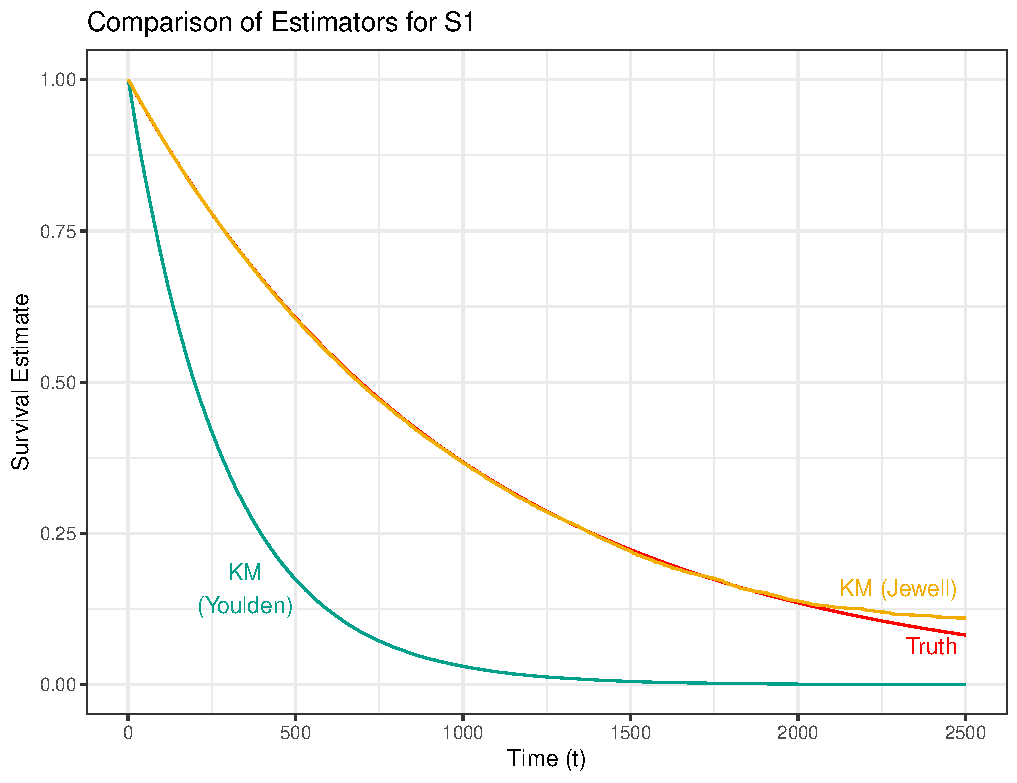
\includegraphics[scale=0.45]{s1_estim_compare}
\vspace{-1.75em}
\captionof{figure}{This figure demonstrates...}
\end{center}

%\vspace{-1.75em}

%\begin{itemize}
  %\itemsep0.05pt
  %\item ...
  %\item ...
  %\item ...
%\end{itemize}

\begin{center}
\vspace*{-0.8cm}  % CHANGE THIS TO ALIGN IMAGES
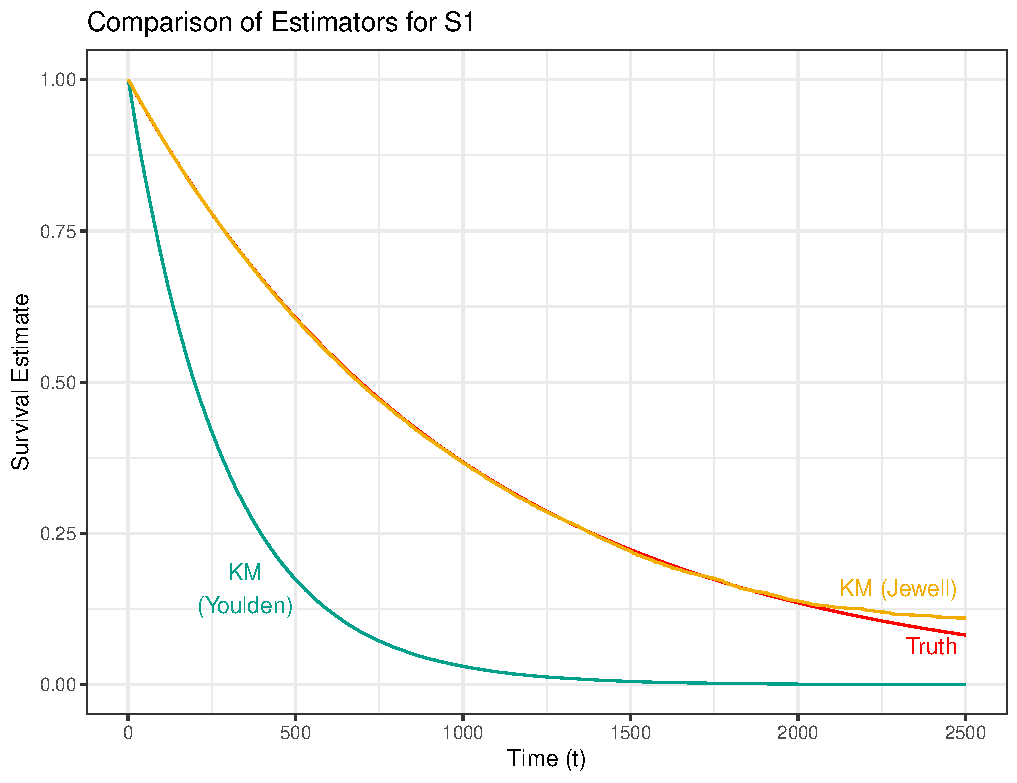
\includegraphics[scale=0.45]{s1_estim_compare}
\vspace{-1.75em}
\captionof{figure}{This figure demonstrates...}
\end{center}

%\vspace{-1.75em}

%\begin{itemize}
  %\itemsep0.05pt
  %\item ...
  %\item ...
  %\item ...
%\end{itemize}

\end{multicols}

\vspace{0.35em}
}

%-------------------------------------------------------------------------------
% METHODS
%-------------------------------------------------------------------------------

\headerbox{Methodology I: The Effect of a Stochastic
  Intervention}{name=method,column=0,span=2,below=overview,
  bottomaligned=references}{
% This block's bottom aligns with the bottom of the conclusion block

\begin{itemize}
  \itemsep1.5pt
  \item Consider $X = (W, A, Y) \sim P_0^X \in \mathcal{M}$, where $W$ is a set
    of baseline covariates, $A$ a treatment, and $Y$ an outcome of interest,
    with no assumptions placed on the statistical model $\mathcal{M}$.
  \item Rather than a deterministic intervention, consider a shift of the
    treatment (i.e., consider a shift of the intervention so that
    $A = A + \delta$ for a user-specified $\delta$).
  %\item As a comparison with the general linear model, the shift $\delta$ may be
    %thought of as a part of the nonparametric analog to the slope of a
    %regression line --- i.e., $\beta^{\text{NP}}_{\text{slope}} =
      %\frac{\mathbb{E}[Y \mid A + \delta] - \mathbb{E}[Y \mid A]}{\delta^2}$.
  \item To protect against violations of the assumption of positivity, the
    shifting mechanism may be made a function of the observed data:
    \[ d(a, w) =
       \begin{cases}
         a + \delta, & a + \delta < u(w) \\
         a, & \text{otherwise}
       \end{cases}
    \]
  \item We consider a simple causal target parameter, introduced in
    \cite{munoz2012population}:
    \begin{equation}
    \Psi(P)(X) = \mathbb{E}_{\text{P}}{\overline{Q}(d(A, W), W)},
    \end{equation}
    \begin{itemize}
      \item for which Wald-style inference is attainable through the efficient
        influence function (EIF), given in \cite{diaz2018stochastic}:
        \begin{equation}
          D(P)(o) = H(a, w){y - \overline{Q}(a, w)} + \overline{Q}(d(a, w), w) -
            \Psi(P)(o),
        \end{equation}
      \item where the auxiliary term, $H(a,w)$, may be expressed as
        \begin{equation}
          H(a,w) = \mathbb{I}(a < u(w)) \frac{g_0(a - \delta \mid w)}{g_0(a
            \mid w)} + \mathbb{I}(a \geq u(w) - \delta).
        \end{equation}
    \end{itemize}
%We obtain Wald-style inference via the limiting distribution:
%$\sqrt{n}(\Psi_n - \Psi) \to N(0, \text{Var}(D(P_0)))$.
\end{itemize}
}

%-------------------------------------------------------------------------------

\end{poster}
\end{document}

